% Section 2 draft: notation and reconciliation of several variables.

\section{Reconciling several variables}
\label{sec:setup}

\subsection{Notation}

We follow the notation of \citet{athanasopoulos2023forecast}, adapted to several variables. Suppose $m$ variables are each observed over the same hierarchy with $n$ series, of which $n_b$ are at the bottom level and $n_a = n - n_b$ are aggregates. For variable $j$, let $\bm{y}_{j,t}$ be the $n$-vector of all its series at time $t$, and $\bm{b}_{j,t}$ the $n_b$-vector of its bottom-level series. Then
\begin{equation}\label{eq:ysb}
  \bm{y}_{j,t} = \bm{S}\bm{b}_{j,t},
  \qquad
  \bm{S} = \begin{bmatrix}\bm{A}\\ \bm{I}_{n_b}\end{bmatrix},
\end{equation}
where the $(n_a \times n_b)$ matrix $\bm{A}$ gives the aggregation constraints. Equivalently, $\bm{C}\bm{y}_{j,t} = \bm{0}$ with $\bm{C} = [\bm{I}_{n_a}\ \ -\bm{A}]$, so that $\bm{C}\bm{S} = \bm{0}$. Figure~\ref{fig:HTS_M.ex} shows a three-level example with $n = 8$ and $n_b = 5$.

\begin{figure}[!htb]
  \centering
  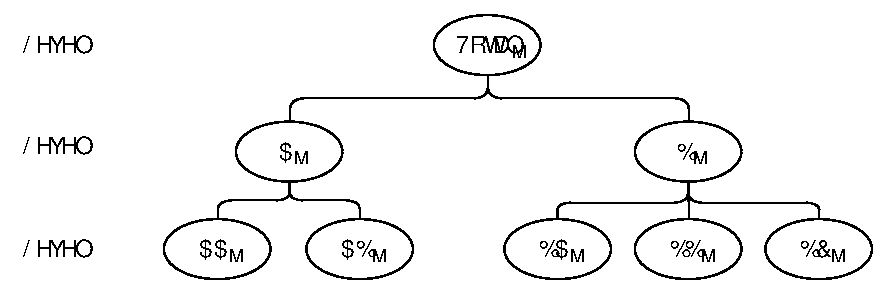
\includegraphics[width=11cm]{Imagens/diagrama_mult.pdf}
  \caption{A hierarchy with three levels, observed for each of $m$ variables.}
  \label{fig:HTS_M.ex}
\end{figure}

Collect the variables in $\bm{Y}_t = [\bm{y}_{1,t}, \dots, \bm{y}_{m,t}]$ and $\bm{B}_t = [\bm{b}_{1,t}, \dots, \bm{b}_{m,t}]$. Stacking the columns gives
\begin{equation}\label{eq:vec}
  \vetor(\bm{Y}_t) = \bm{S}_*\vetor(\bm{B}_t),
  \qquad
  \bm{S}_* = \bm{I}_m \otimes \bm{S},
\end{equation}
with constraint matrix $\bm{C}_* = \bm{I}_m \otimes \bm{C}$. The stacked summing matrix is block diagonal: no constraint links one variable to another. This distinguishes the setting from a grouped hierarchy, where the categories of a grouping variable (such as travel purpose in the Australian tourism data of \citealp{wickramasuriya2019optimal}) are linked by aggregation constraints because their total is itself observed and forecast.

\subsection{Forecast reconciliation}

Let $\widehat{\bm{y}}_{T+h|T}$ be the stacked $h$-step base forecasts of all $mn$ series, produced without regard to the constraints, and let $\bm{W}_h$ be the covariance matrix of their errors. Linear reconciliation maps the base forecasts to coherent forecasts $\widetilde{\bm{y}}_{T+h|T} = \bm{S}_*\bm{P}\widehat{\bm{y}}_{T+h|T}$ for some matrix $\bm{P}$ with $\bm{P}\bm{S}_* = \bm{I}$. The minimum trace (MinT) choice \citep{wickramasuriya2019optimal} minimises the trace of the reconciled error covariance and gives
\begin{equation}\label{eq:mint}
  \widetilde{\bm{y}}_{T+h|T} = \bm{S}_*(\bm{S}_*'\bm{W}_h^{-1}\bm{S}_*)^{-1}\bm{S}_*'\bm{W}_h^{-1}\widehat{\bm{y}}_{T+h|T}
  = \big[\bm{I} - \bm{W}_h\bm{C}_*'(\bm{C}_*\bm{W}_h\bm{C}_*')^{-1}\bm{C}_*\big]\widehat{\bm{y}}_{T+h|T},
\end{equation}
the second form being the zero-constrained representation of \citet{di2023cross}. Applied to the stacked system this is ordinary MinT with summing matrix $\bm{S}_*$; we call it \emph{joint} reconciliation. \emph{Separate} reconciliation applies MinT to each variable on its own, using only the diagonal block of $\bm{W}_h$ for that variable. Joint reconciliation can use the cross-variable blocks of $\bm{W}_h$, and it is natural to expect it to be more accurate when the variables' forecast errors are correlated. Section~\ref{sec:theory} shows when that expectation holds.

In practice $\bm{W}_h$ is unknown. Following \citet{wickramasuriya2019optimal}, we set $\bm{W}_h = k_h\widehat{\bm{W}}_1$, where $\widehat{\bm{W}}_1$ is the shrinkage estimator
\begin{equation}\label{eq:shrink}
  \widehat{\bm{W}}_1 = \lambda\widehat{\bm{W}}_{1,D} + (1 - \lambda)\widehat{\bm{W}}_{1,S},
\end{equation}
$\widehat{\bm{W}}_{1,S}$ is the sample covariance matrix of the one-step in-sample residuals, $\widehat{\bm{W}}_{1,D}$ is its diagonal, and the intensity $\lambda$ is estimated as in \citet{schafer2005shrinkage}. The scale $k_h$ cancels from \eqref{eq:mint}. For separate reconciliation the estimator is applied to each variable's residuals on its own, so each variable has its own shrinkage intensity.
